% q4_eda.tex - Question 4 parts 1(a) 1(b) (OWNER: D) - prose integrated verbatim from report/Q4_D_report_final.md
\section{Question 4: What Makes a Hit? Exploring QQ Music}

\subsection*{4.1(a) Data and exploratory analysis}

The supplied dataset contains 844 song records. We used C's trial\_v1 working data. One invalid text value in streams was recorded as missing. We selected six candidate predictors and one response variable, retaining 843 records with complete values for these variables. Records with a blank key were retained because key was not included in this analysis. All the figures, summary statistics, correlations and variance inflation factors below are based on the same 843 records.

\begin{table}[htbp]
  \centering
  \small
  \caption*{Table Q4-D1: Descriptive statistics of the analysis variables ($n = 843$).}
  \setlength{\tabcolsep}{3.5pt}
  \begin{tabular}{lrrrrrrrr}
    \toprule
    Variable & $N$ & Mean & SD & Min & Q1 & Median & Q3 & Max \\
    \midrule
    Streams (million) & 843 & 536.062 & 584.495 & 0.003 & 147.040 & 301.052 & 703.736 & 3703.895 \\
    ln(streams) & 843 & 19.541 & 1.169 & 7.924 & 18.806 & 19.523 & 20.372 & 22.033 \\
    QQ playlist inclusions & 843 & 5531.019 & 8268.126 & 31 & 895 & 2313 & 6077 & 52898 \\
    ln(QQ playlist inclusions) & 843 & 7.774 & 1.342 & 3.434 & 6.797 & 7.746 & 8.712 & 10.876 \\
    Artist count & 843 & 1.515 & 0.842 & 1 & 1 & 1 & 2 & 8 \\
    Release year & 843 & 2018.053 & 11.067 & 1942 & 2020 & 2022 & 2022 & 2023 \\
    Danceability (0--100) & 843 & 66.471 & 14.850 & 23 & 56 & 68 & 78 & 96 \\
    Energy (0--100) & 843 & 63.745 & 16.692 & 9 & 53 & 65 & 76.5 & 97 \\
    Acousticness (0--100) & 843 & 27.000 & 26.334 & 0 & 5 & 17 & 43 & 97 \\
    \bottomrule
  \end{tabular}
\end{table}

Table Q4-D1 shows that the mean total streams is 536.062 million and the median is 301.052 million. Figure Q4-D1 shows that the distribution is strongly right-skewed, with a small number of songs having very high stream counts. After applying a natural logarithm transformation, the long upper tail is compressed and most observations form a more compact cluster (see Figure Q4-D2). However, a few very low values remain in the left tail. These records were retained. The histogram alone does not indicate whether the regression assumptions are met.

\begin{figure}[htbp]
  \centering
  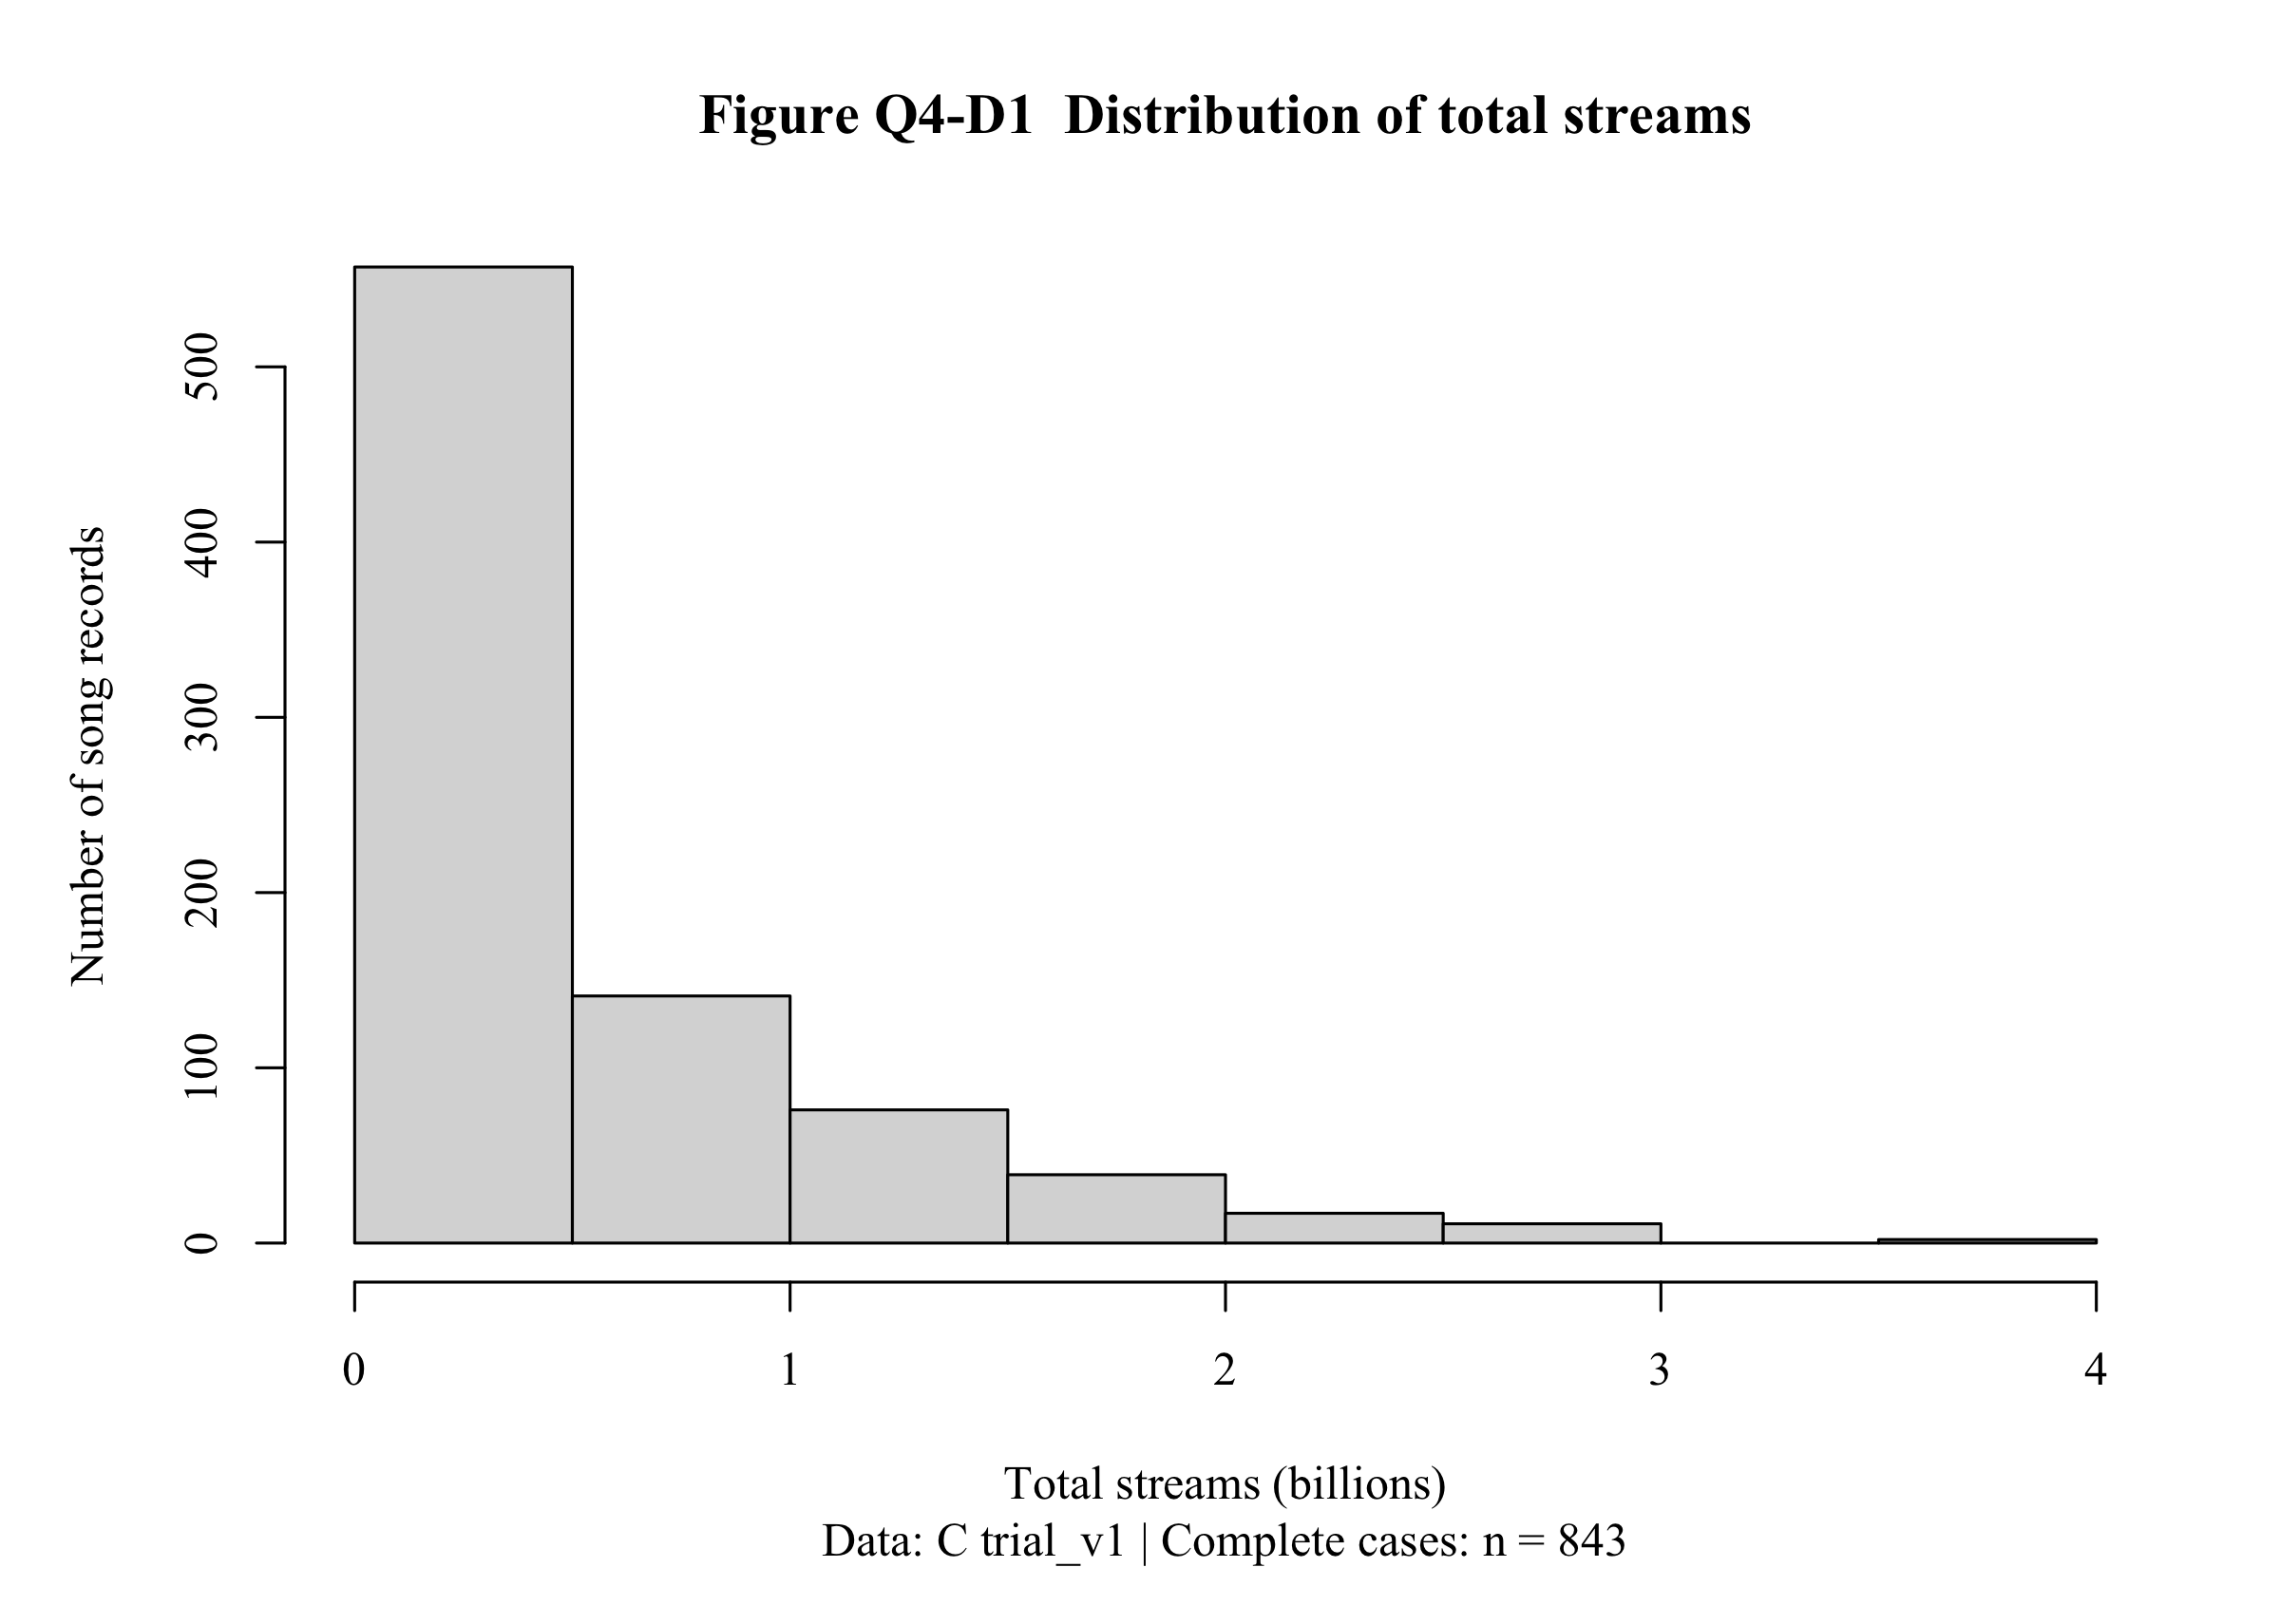
\includegraphics[width=0.8\textwidth]{Q4_D_Figure_01.png}
  \caption*{Figure Q4-D1: Distribution of total streams.}
\end{figure}

\begin{figure}[htbp]
  \centering
  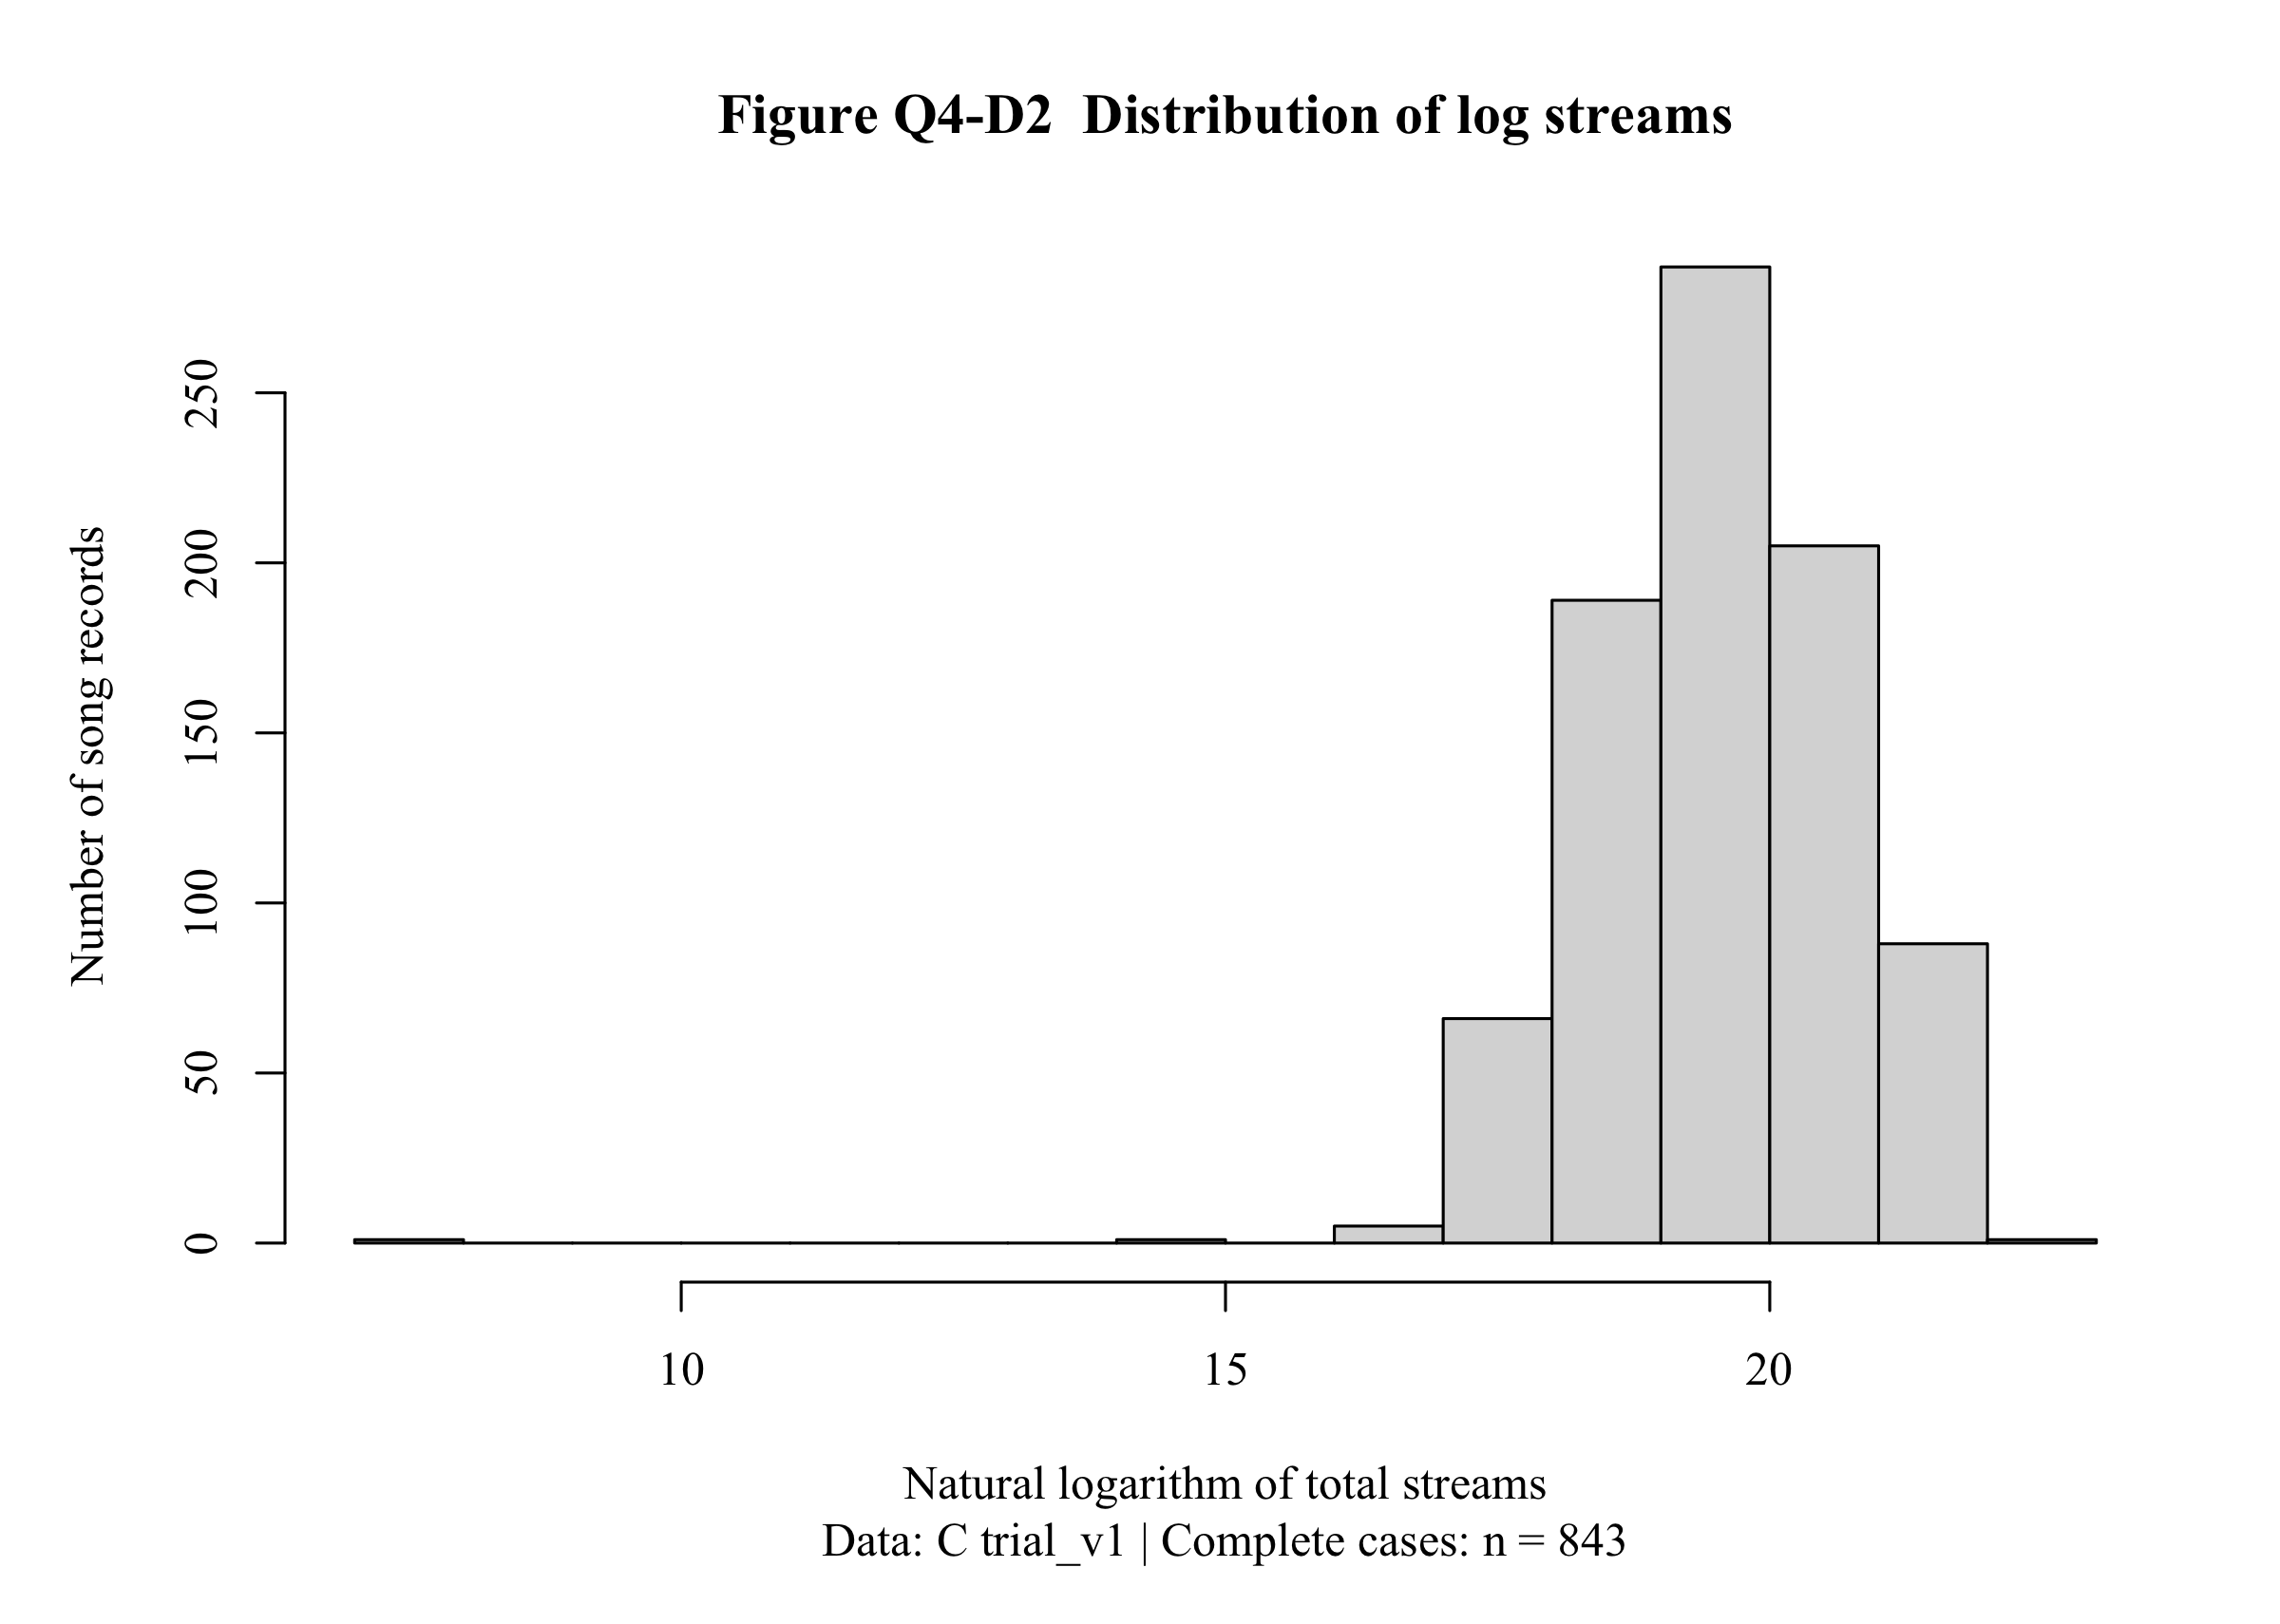
\includegraphics[width=0.8\textwidth]{Q4_D_Figure_02.png}
  \caption*{Figure Q4-D2: Distribution of log streams.}
\end{figure}

Figure Q4-D3 shows a positive but curved association between QQ playlist inclusions and log streams. The pattern is steeper at lower playlist counts and flatter at higher ones. When playlist inclusions are also transformed using the natural logarithm, the main pattern resembles a positive straight line more closely (see Figure Q4-D4). This suggests that log playlist inclusions should be considered in the candidate model. However, it does not establish the adjusted association, so model comparison and residual diagnostics are still needed.

\begin{figure}[htbp]
  \centering
  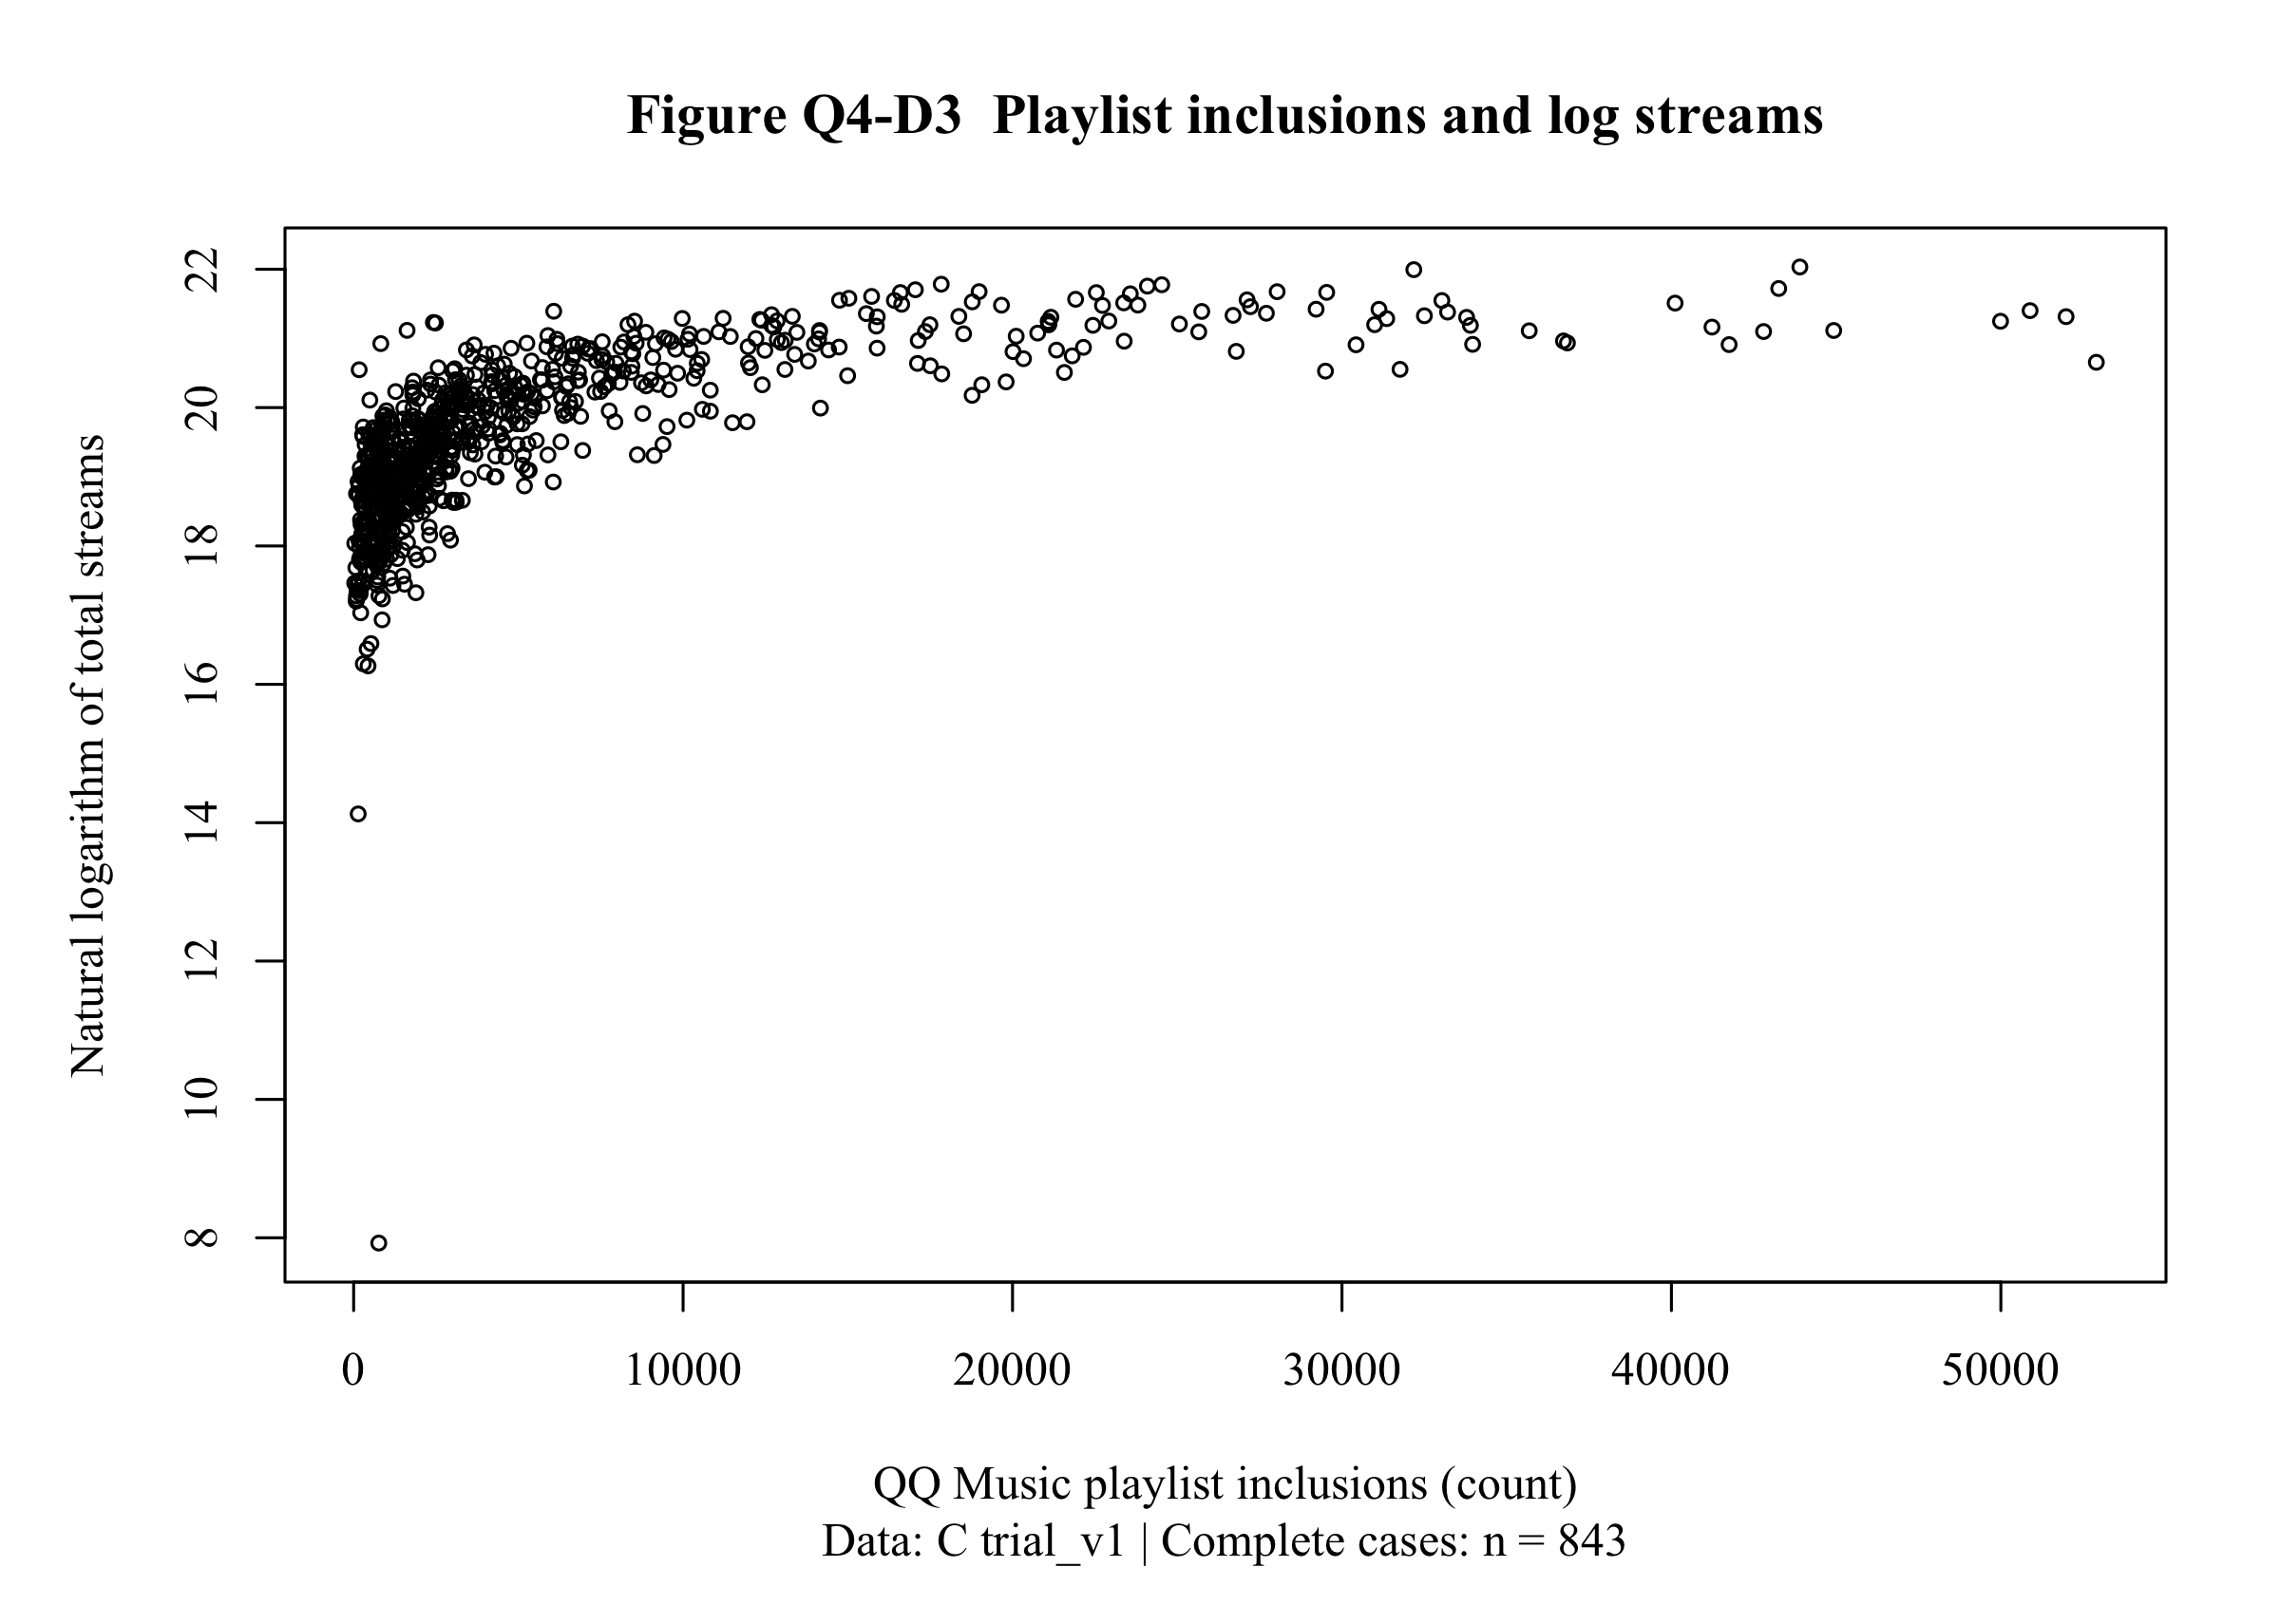
\includegraphics[width=0.8\textwidth]{Q4_D_Figure_03.png}
  \caption*{Figure Q4-D3: QQ playlist inclusions and log streams.}
\end{figure}

\begin{figure}[htbp]
  \centering
  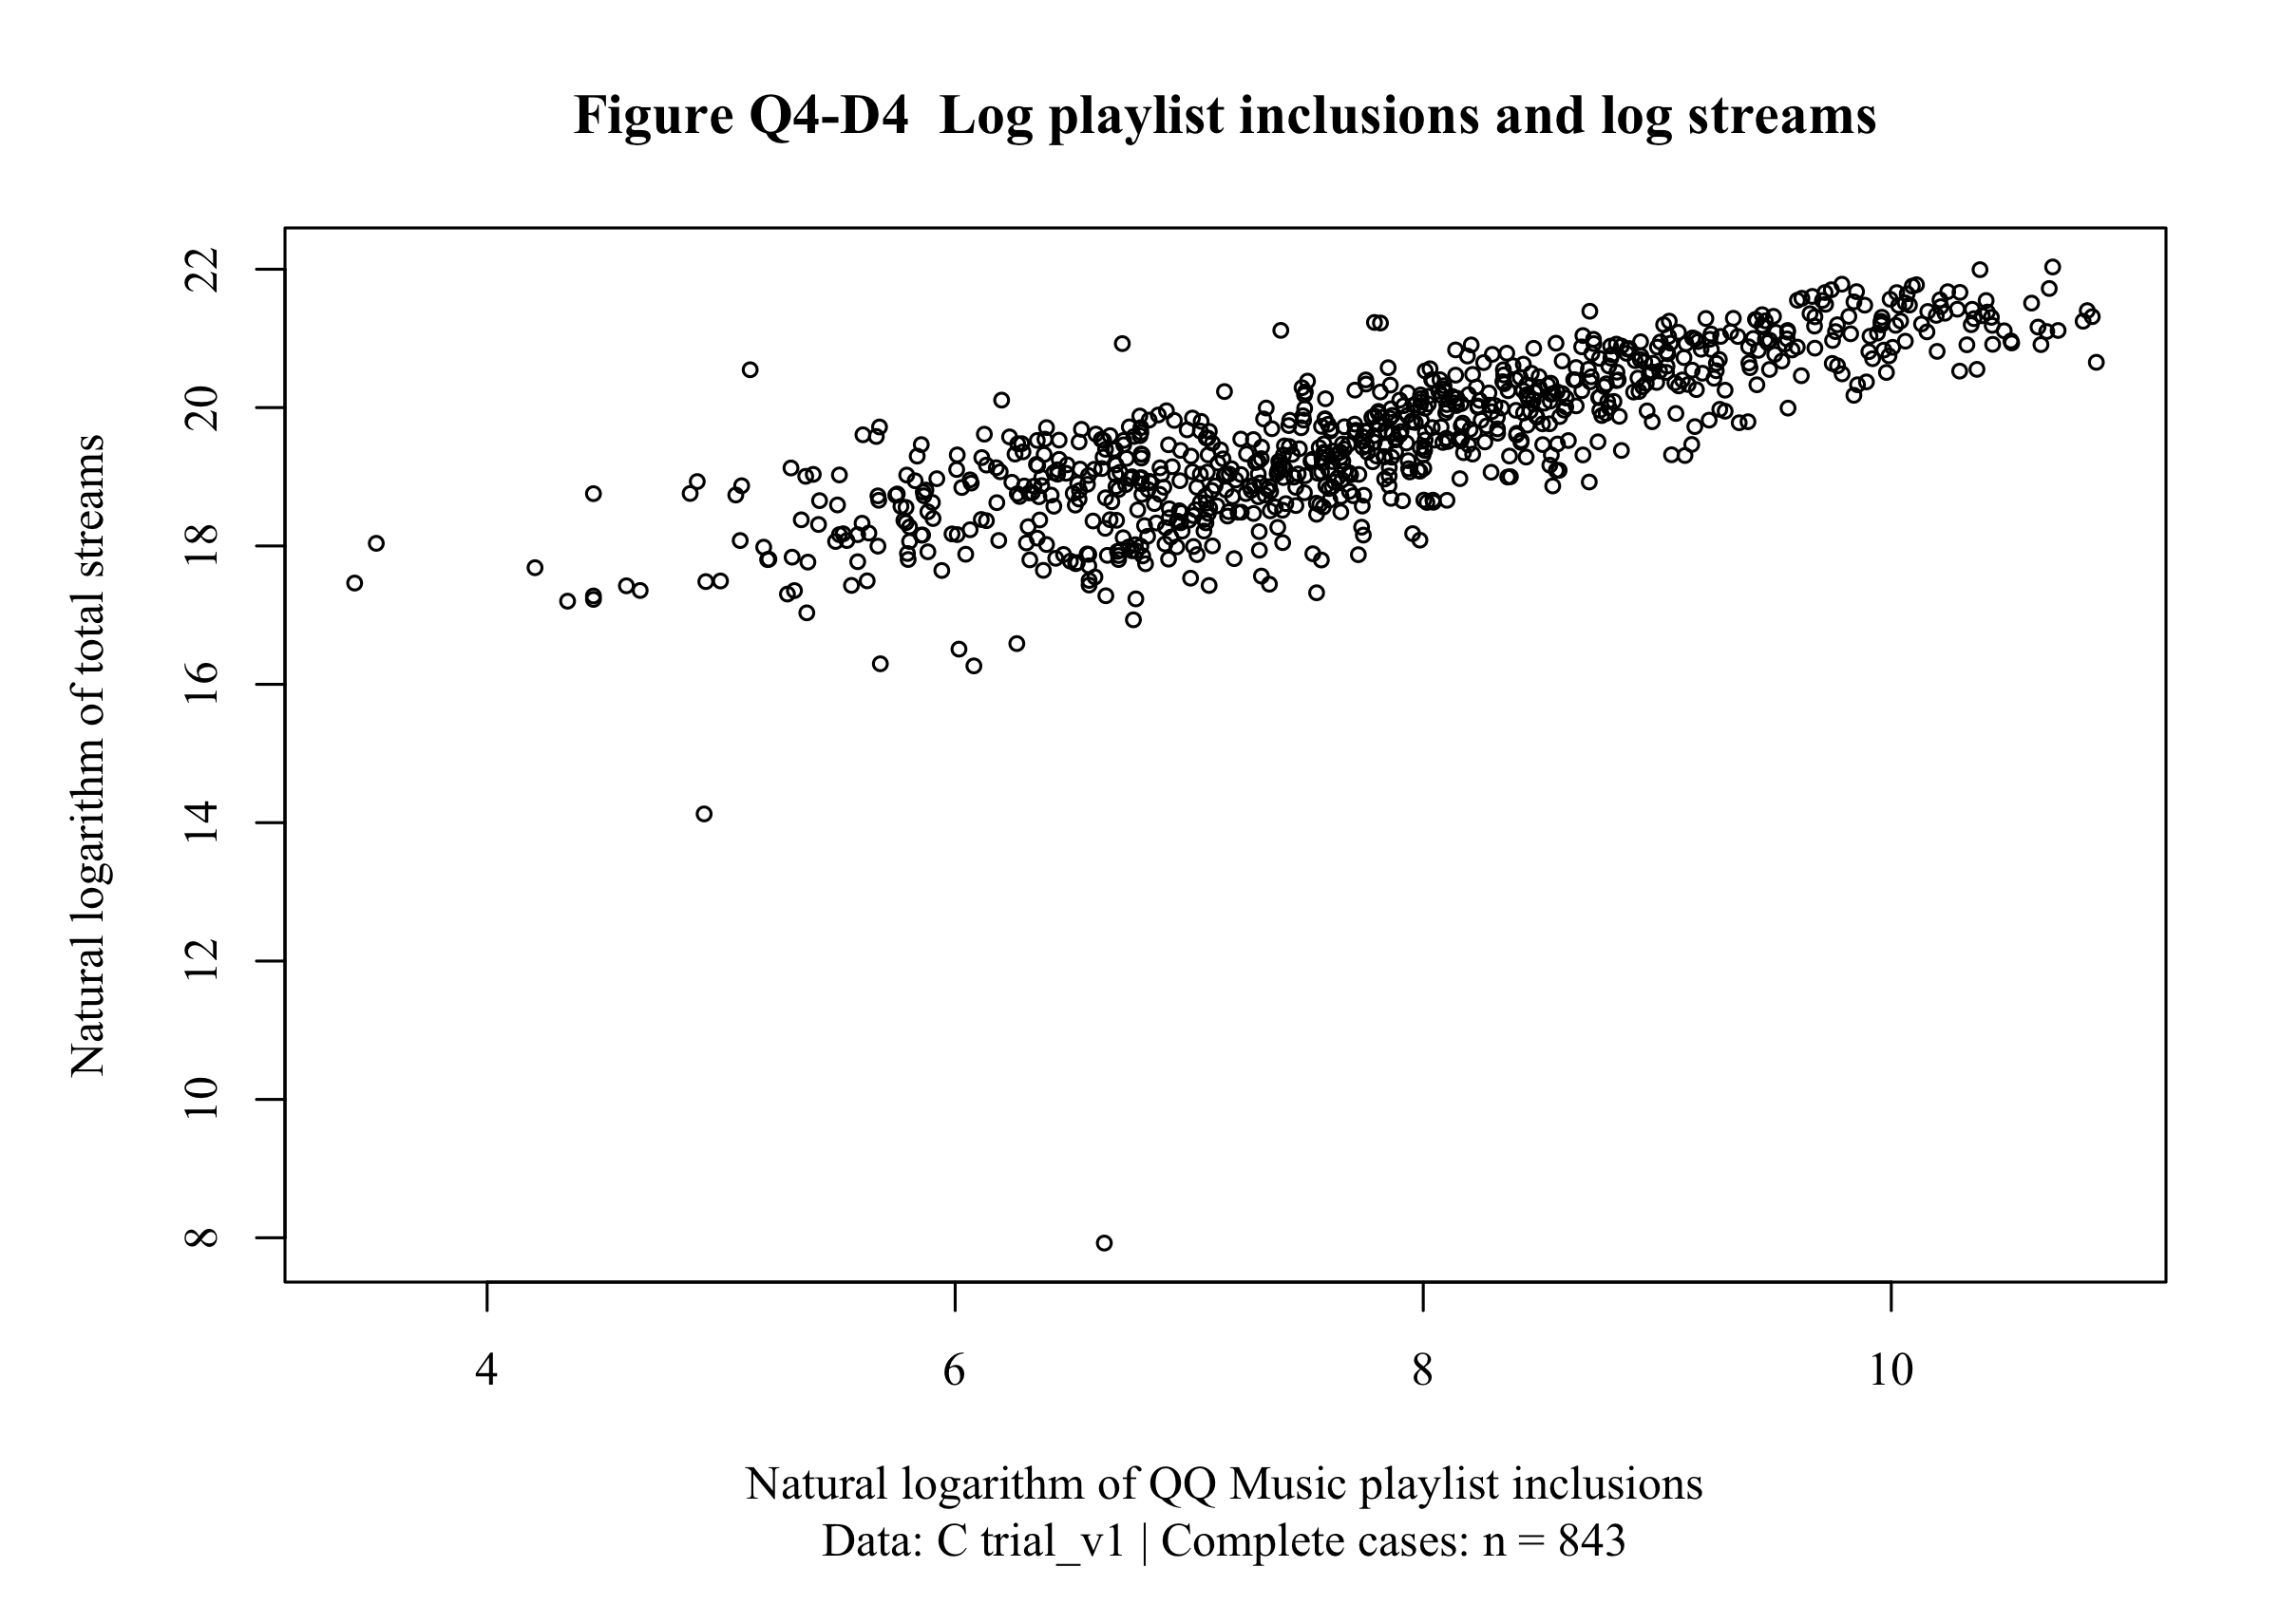
\includegraphics[width=0.8\textwidth]{Q4_D_Figure_04.png}
  \caption*{Figure Q4-D4: Log playlist inclusions and log streams.}
\end{figure}

Figure Q4-D5 shows a negative association between energy and acousticness. Their Pearson correlation is $-0.595$. Table Q4-D1 shows that the median values are 68.000 for danceability, 65.000 for energy and 17.000 for acousticness. These features are recorded on 0--100 scales. While these results describe the sample, they do not demonstrate that any feature causes higher streams.

\begin{figure}[htbp]
  \centering
  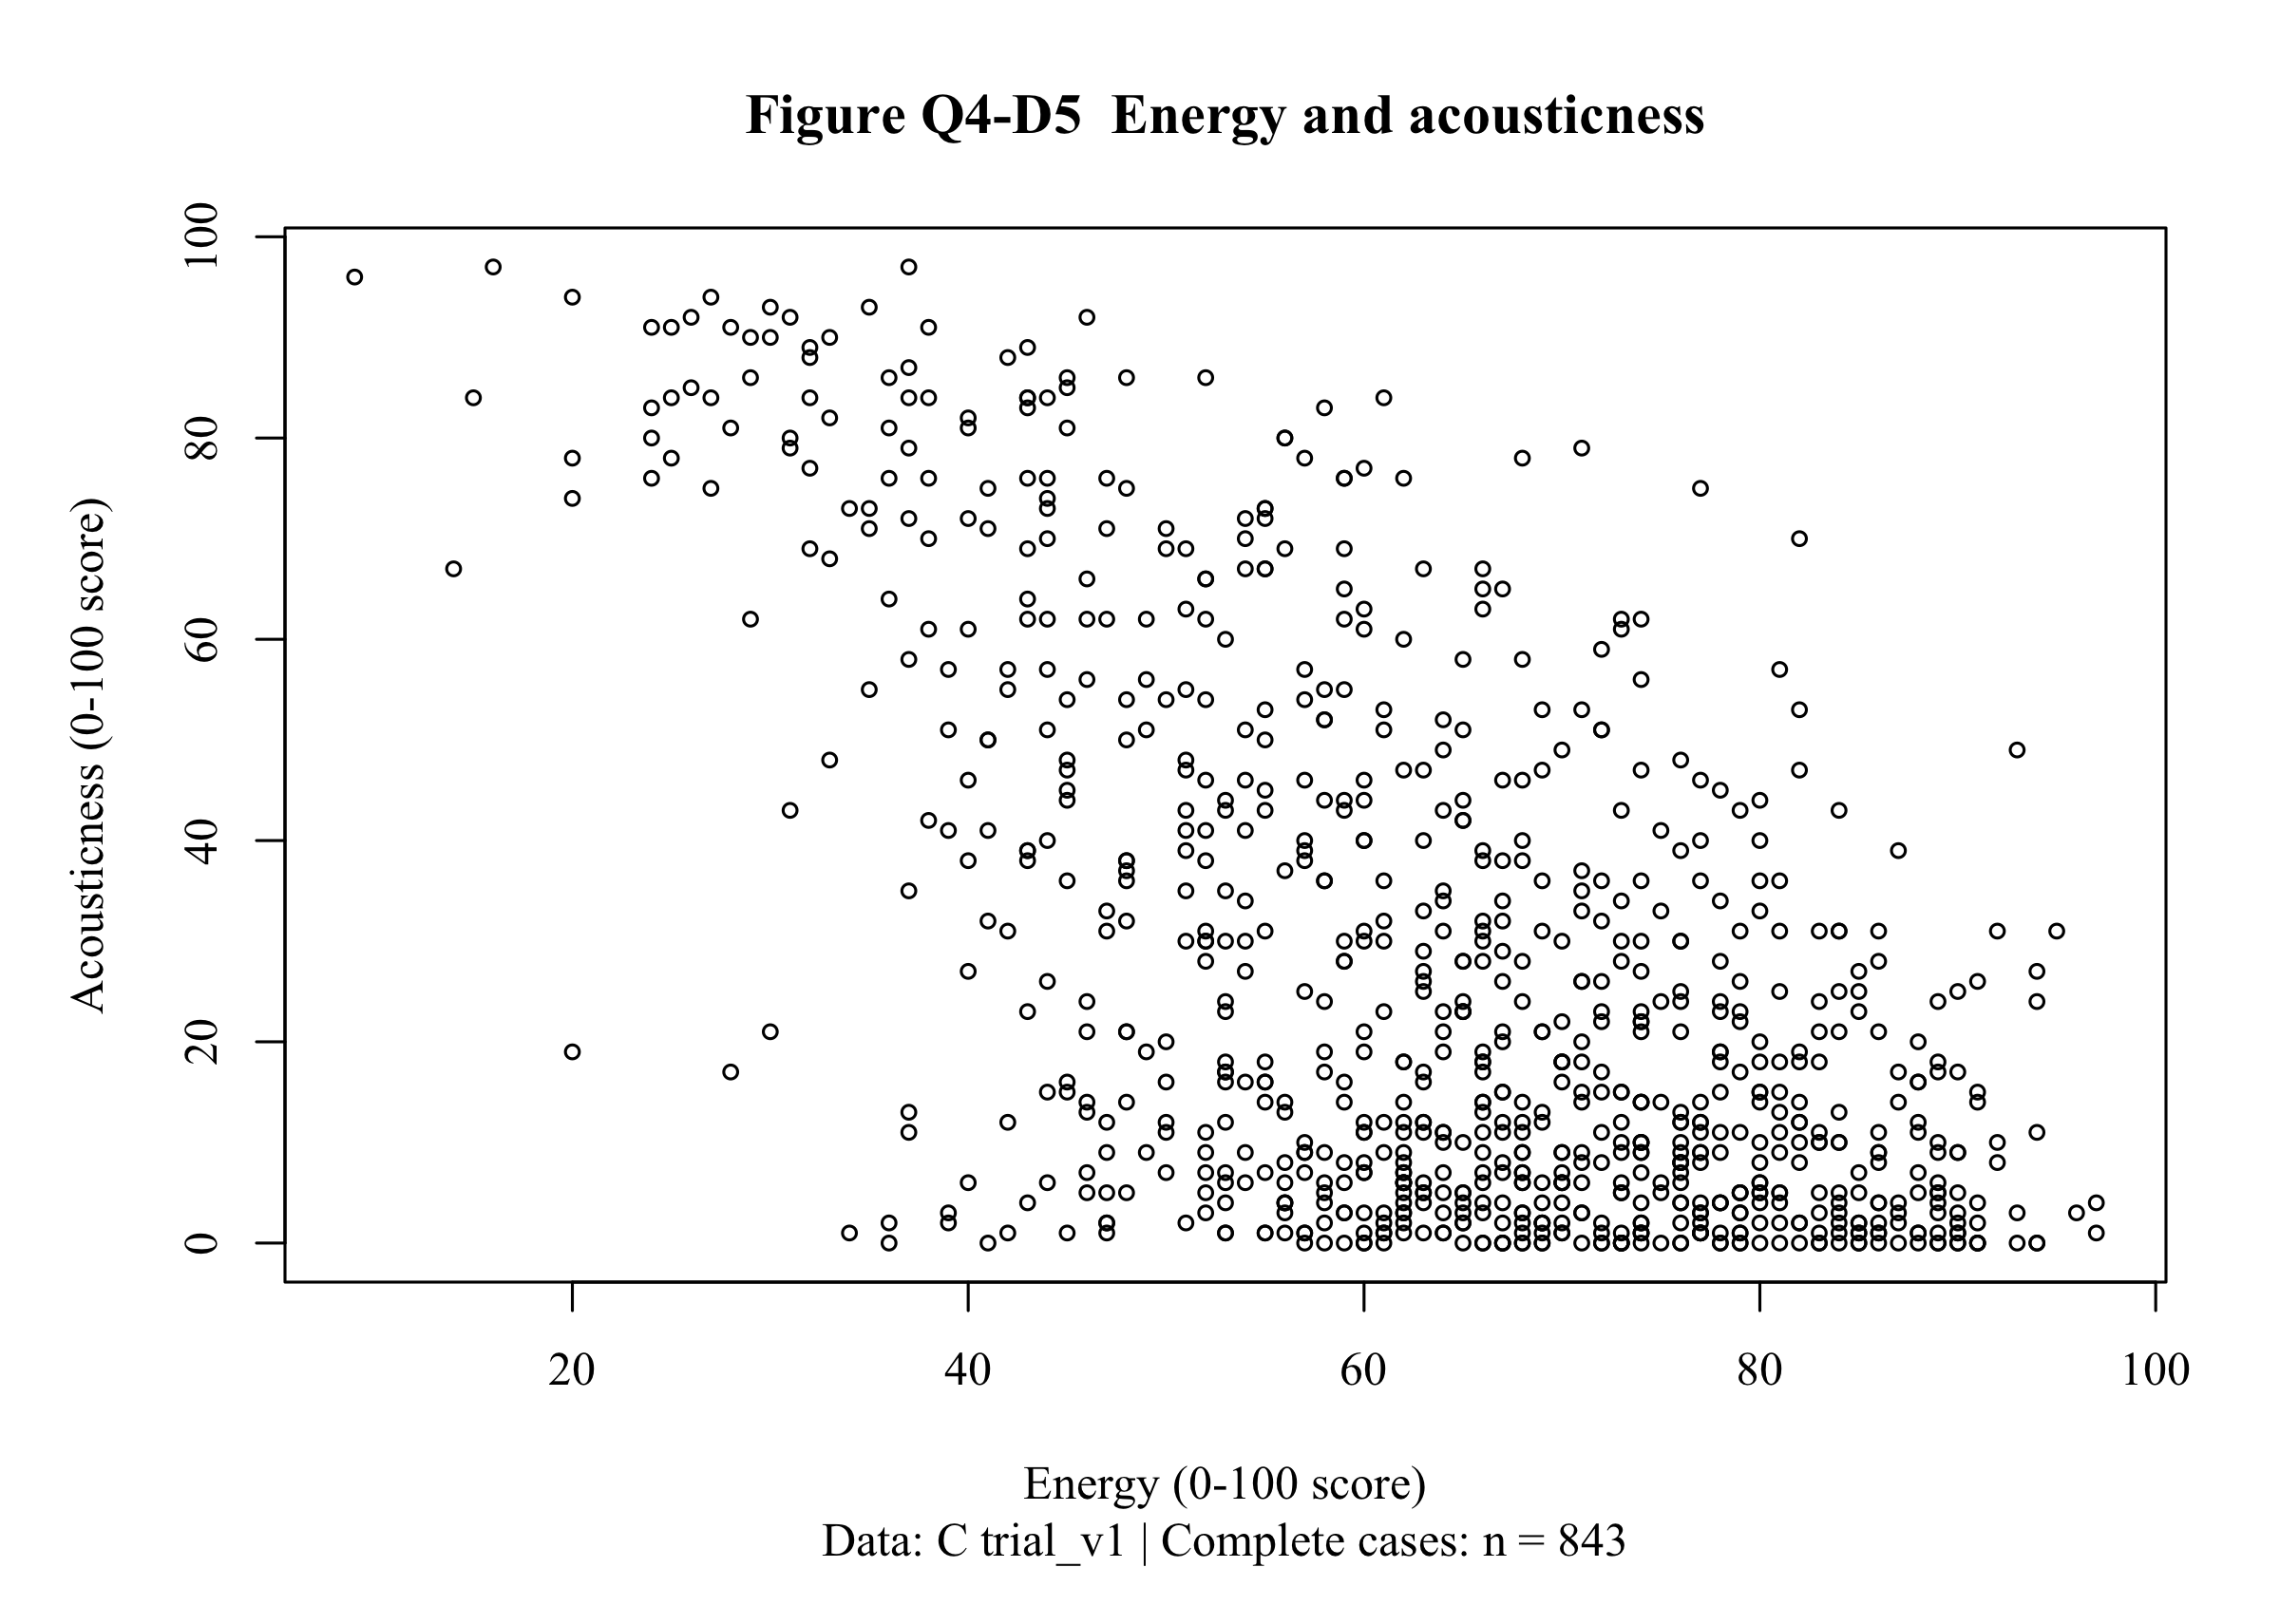
\includegraphics[width=0.8\textwidth]{Q4_D_Figure_05.png}
  \caption*{Figure Q4-D5: Energy and acousticness.}
\end{figure}

\subsection*{4.1(b) Research question and relevance}

Our research question is: How is QQ Music playlist inclusion associated with the natural logarithm of cumulative song streams, after accounting for artist count, release year, danceability, energy and acousticness?

The response variable is log(streams). QQ playlist inclusion is the main predictor, with its log transformation supported by the exploratory plots. The other candidate predictors are artist count, release year, danceability, energy, and acousticness. Playlist inclusion is important to the QQ Music team as a source of exposure. Studying its association with streams while accounting for selected song characteristics can inform the evaluation of playlist promotion. However, popular songs may also be more likely to be included in playlists. Therefore, the observed association cannot be interpreted as the effect of adding a song to a playlist.
